
\newpage
\subsection{Scalar AES Acceleration}
\label{sec:scalar:aes}

This section details proposals for acceleration of
the AES block cipher \cite{nist:fips:197} within a scalar RISC-V core,
obeying the two-read-one-write constraint on general purpose register
file accesses.

\subsubsection{RV32 Instructions}
\label{sec:scalar:aes:rv32}

\begin{cryptoisa}
saes32.encs      rd, rs1, rs2, bs // Encrypt: SubBytes
saes32.encsm     rd, rs1, rs2, bs // Encrypt: SubBytes & MixColumns
saes32.decs      rd, rs1, rs2, bs // Decrypt: SubBytes
saes32.decsm     rd, rs1, rs2, bs // Decrypt: SubBytes & MixColumns
\end{cryptoisa}

These instructions are a very lightweight proposal, derived from
\cite{MJS:LWAES:20}.
They are designed to enable a partial T-Table based implementation
of AES in hardware, where the SubBytes, ShiftRows and MixColumns
transformations are all rolled into a single instruction, with the
per-byte results then accumulated.
The {\tt bs} immediate operand is a 2-bit {\em Byte Select}, and indicates
which byte of the input word is operated on.
SAIL Model code for each instruction is found in figure
\ref{fig:pseudo:aes:rv32}.

These instructions use the Equivalent Inverse Cipher
construction \cite[Section 5.3.5]{nist:fips:197}.
This affects the computation of the KeySchedule, as shown in
\cite[Figure 15]{nist:fips:197}.

\begin{figure}[h]
\lstinputlisting[language=sail,firstline=66,lastline=82]{../sail/riscv_insts_crypto_rv32.sail}
\caption{SAIL specification for the lightweight AES instructions targeting the
RV32 base architecture.}
\label{fig:pseudo:aes:rv32}
\end{figure}

\note{
The SM4 (see Section \ref{sec:scalar:sm4}) and RV32 AES 
instructions are designed to share much of their data-path, and
can be implemented with much logic shared  between their SBoxes
in particular.
}


% ------------------------------------------------------------

\newpage
\subsubsection{RV64 Instructions}
\label{sec:scalar:aes:rv64}

\begin{cryptoisa}
saes64.ks1   rd, rs1, rcon // KeySchedule: SubBytes, Rotate, Round Const
saes64.ks2   rd, rs1, rs2  // KeySchedule: XOR summation
saes64.imix  rd, rs1       // KeySchedule: InvMixColumns for Decrypt
saes64.encsm rd, rs1, rs2  // Round:    ShiftRows,    SubBytes,    MixColumns
saes64.encs  rd, rs1, rs2  // Round:    ShiftRows,    SubBytes
saes64.decsm rd, rs1, rs2  // Round: InvShiftRows, InvSubBytes, InvMixColumns
saes64.decs  rd, rs1, rs2  // Round: InvShiftRows, InvSubBytes
\end{cryptoisa}

These instructions are for RV64 only.
They implement the SubBytes, ShiftRows and MixColumns transformations of AES.
Each round instruction takes two 64-bit registers as input, representing
the 128-bit state of the AES cipher, and outputs one 64-bit
result, i.e. half of the next round state.
The byte mapping of input register values to AES state and output register
values is shown in \figref{aes:rv64:mapping}.
Pseudocode for the instructions is illustrated in
\figref{pesudo:aes:rv64}.

\begin{itemize}

\item
The
\mnemonic{saes64.ks1}/\mnemonic{saes64.ks2}
instructions are used in the encrypt KeySchedule.
\mnemonic{saes64.ks1} implements the rotation, SubBytes and Round Constant
addition steps.
\mnemonic{saes64.ks2} implements the remaining {\tt xor} operations.

\item
The
\mnemonic{saes64.imix}
instruction applies the inverse MixColumns
transformation to two columns of the state array, packed into a single
64-bit register.
It is used to create the inverse cipher KeySchedule, according to
the equivalent inverse cipher construction in
\cite[Page 23, Section 5.3.5]{nist:fips:197}.

\item
The \mnemonic{saes64.encsm}/\mnemonic{saes64.decsm} instructions perform the
(Inverse) SubBytes, ShiftRows and MixColumns Transformations.

\item
The \mnemonic{saes64.encs}/\mnemonic{saes64.decs} instructions perform the
(Inverse) SubBytes and ShiftRows Transformations.
They are used for the last round only.

\item
Computing the next round state uses two instructions.
The high or low 8 bytes of the next state are selected by swapping the order
of the source registers.
The following code snippet shows one round of the AES block encryption.
{\tt t0} and {\tt t1} hold the current round state.
{\tt t2} and {\tt t3} hold the next round state.
\begin{lstlisting}
saes64.encsm t2, t0, t1 // ShiftRows, SubBytes, MixColumns bytes 0..7
saes64.encsm t3, t1, t0 // "          "         "          "     8..15
\end{lstlisting}
\end{itemize}

This proposal requires $6$ instructions per AES round:
$2$ \mnemonic{ld} instructions to load the round key,
$2$ \mnemonic{xor} to add the round key to the current state
and
$2$ of the relevant AES encrypt/decrypt instructions to perform the
    SubBytes, ShiftRows and MixColumns round functions.
An un-rolled AES-128 block encryption with an offline KeySchedule
hence requires $69$ instructions in total.

These instructions are amenable to macro-op fusion.
The recommended sequences are:
\begin{lstlisting}[language=pseudo]
saes64.encsm rd1, rs1, rs2 // Different destination registers,
saes64.encsm rd2, rs2, rs1 // identical source registers with swapped order.
\end{lstlisting}
This is similar to the recommended \mnemonic{mulh}, \mnemonic{mul}
sequence in the M extension to compute a full $32*32->64$ bit
multiplication result \cite[Section 7.1]{riscv:spec:user}.

Unlike the $32$-bit AES instructions, the $64$-bit variants
{\em do not} use the Equivalent Inverse Cipher
construction \cite[Section 5.3.5]{nist:fips:197}.

\begin{figure}[h]
\centering
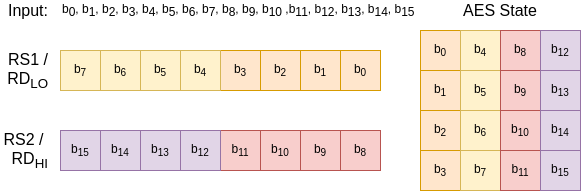
\includegraphics[width=0.8\textwidth]{diagrams/aes-rv64-state.png}
\caption{
Mapping of AES state between input and output registers for the round
instructions.
{\tt Rout1} is given by \mnemonic{saes64.encsm rd, rs1, rs2},
and
{\tt Rout2}          by \mnemonic{saes64.encsm rd, rs2, rs1}.
The {\tt [Inv]ShiftRows} blocks show how to select the relevant $8$ bytes
for further processing from the concatenation {\tt rs2 || \tt rs1}.
}
\label{fig:aes:rv64:mapping}
\end{figure}

\begin{figure}[h!]
\begin{lstlisting}[language=pseudo]
saes64.ks1(rs1,enc_rcon):      // KeySchedule: SubBytes, Rotate, Round Const
    temp.32   = rs1.32[1]
    rcon      = 0x0
    if(enc_rcon != 0xA):
        temp.32 = ROTR32(temp.32, 8)
        rcon    = AESRoundConstants.8[enc_rcon]
    temp.8[i] = AESSBox(temp.8[i])  for i=0..3
    temp.8[0] = temp.8[i  ] ^ rcon
    rd.64     = {temp.32, temp.32}

saes64.ks2(rs1,rs2):           // KeySchedule: XOR
    rd.32[0]  = rs1.32[1] ^ rs2.32[0]
    rd.32[1]  = rs1.32[1] ^ rs2.32[0] ^ rs2.32[1]

saes64.imix(rs1):              // Inverse MixColumns
    rd.32[0]  = InvAESMixColumn(rs1.32[0])
    rd.32[1]  = InvAESMixColumn(rs1.32[1])

saes64.enc(rs1, rs2, mix):     // SubBytes, ShiftRows, MixColumns
    t1.128    = AESShiftRows(rs2 || rs1)
    t2.64     = t1.64[0]
    t3.8[i]   = AESSBox(t2.8[i]) for i=0..7
    rd.32[0]  = AESMixColumn(t3.32[0]) if mix else t3.32[0]
    rd.32[1]  = AESMixColumn(t3.32[1]) if mix else t3.32[1]

saes64.dec(rs1, rs2, mix):     // InvSubBytes, InvShiftRows, InvMixColumns
    t1.128    = InvAESShiftRows(rs2 || rs1)
    t2.64     = t1.64[0]
    t3.8[i]   = InvAESSBox(t2.8[i]) for i=0..7
    rd.32[0]  = InvAESMixColumn(t3.32[0]) if mix else t3.32[0]
    rd.32[1]  = InvAESMixColumn(t3.32[1]) if mix else t3.32[1]
\end{lstlisting}
\caption{
RV64 AES instruction pseudocode.
}
\label{fig:pesudo:aes:rv64}
\end{figure}

